\documentclass[a4paper,12pt]{article}

%Class
	%\documentclass[a4paper,12pt]{article}

%Packages
	\usepackage{amsmath}					% Standard maths
	\usepackage{amssymb}					% Standard maths
	\usepackage{amsthm}						% Standard maths
	\usepackage{thmtools, thm-restate}% Theorem styles
	\usepackage{mathtools}
	\usepackage[newzealand]{babel}% Date/time in British format (yes, I know it says NZ)
	\usepackage{datetime}					% Date/time
	\usepackage{multirow}					% For stacked subscripts
	\usepackage{xcolor}						% For colour!
	\usepackage[normalem]{ulem}		% For strikeout
	\usepackage{isomath}
	\usepackage{fancyhdr}					% For the headers
	\usepackage{mfirstuc}					% For the headers
	\usepackage[hmargin=1in,top=0.8in,bottom=1in]{geometry} % Page margins more reasonable
	\usepackage{graphicx}					% For including graphics
	%\usepackage{float}						% For something
	\usepackage{enumitem}					% For numbering tweaks
	\usepackage{pgfplots}
	\usepackage[margin=15pt,font={footnotesize},labelfont=bf,format=hang]{caption}
\usepackage[margin=15pt,font={footnotesize},labelfont=bf,format=hang]{subcaption}
	\usepackage{url}
	\usepackage[hidelinks]{hyperref}	% For hyperlinks
	\usepackage{breakurl}
	\usepackage{cleveref}
	\usepackage[scaled=.92]{helvet}
	\newbool{show_question}
	\newbool{show_solution}
	\newcommand{\solutioninheading}{\ifbool{show_solution}{: SOLUTIONS}{}}
	\usepackage{pgfplots}
\newcommand{\ep}{\varepsilon}

\makeatletter 
\newcommand\mynobreakpar{\par\nobreak\@afterheading} 
\makeatother

    \newcommand{\question}[3]{
    	\item \textbf{#1} \mynobreakpar \nobreak \medskip % Title
    	%
    	\ifbool{show_question}{\nobreak#2}{} % Question
    	%
    	%
    	\ifbool{show_question}{\ifbool{show_solution}{\par\medskip\textbf{Solution:}}{}}{} % Both
    	\ifbool{show_solution}{#3}{} % Answer
    }			

%MATHEMATICAL SHORTCUTS
%Two and three-part definitions
	\newcommand{\twopartdef}[4]
	{	\left\{
			\begin{array}{ll}
				#1 & \mbox{if } #2 \\
				#3 & \mbox{if } #4
			\end{array}
		\right.}
%	\newcommand{\threepartdef}[6]
%	{	\left\{
%			\begin{array}{ll}
%				#1 & \mbox{if } #2 \\
%				#3 & \mbox{if } #4 \\
%				#5 & \mbox{if } #6
%			\end{array}
%		\right.}
%Blackboard bold	
	\newcommand{\N}{{\mathbb N}} 
	\newcommand{\R}{{\mathbb R}} 
	\newcommand{\C}{{\mathbb C}} 
	%Curly letters
%	\newcommand{\E}{{\mathcal E}}	
%	\newcommand{\F}{{\mathcal F}} 
%	\newcommand{\Null}{{\mathcal N}} 
%	\newcommand{\R}{\mathcal{R}} 
%	\newcommand{\Z}{\mathcal{Z}} 
%Uprights
	\newcommand{\D}{{\mathrm D}}
	\renewcommand{\d}{{\mathrm d}}
%Easy Greeks
%	\def\a{\alpha}
%	\def\g{\gamma}
%	\newcommand{\e}{{\varepsilon}}
%	\newcommand{\la}{{\lambda}}  
%	\newcommand{\om}{{\Omega}}
	\renewcommand{\epsilon}{\varepsilon}
	
%Vector operators
	\def \p {\partial}
	\newcommand{\del}{{\nabla}}
	\newcommand{\grad}{{\nabla}}
    \newcommand{\vdel}{\boldsymbol{\nabla}}
    \newcommand{\vgrad}{\boldsymbol{\nabla}}
    \newcommand{\vnabla}{\boldsymbol{\nabla}}
	\newcommand{\cross}{{\times}}
	\newcommand{\Lap}{{\nabla^2}} 
%Arrows
%	\newcommand{\goesto}[1]{\xrightarrow[#1]{}}
%hats
%	\newcommand{\nhat}{\widehat{\v{n}}}
%	\newcommand{\shat}{\widehat{\v{s}}}
	\renewcommand{\hat}{\widehat}
%Note to self
%	\newcommand{\note}[1]{[\textbf{\textsl{\MakeUppercase{#1}}}]}
	
%Stress tensor
%	\newcommand{\T}{\vg{\sigma}}

% Vectors, quaternions etc.
\renewcommand{\v}[1]{\mathbfit{#1}}      % Generic vector
\newcommand{\vc}[1]{\bm{\mathcal{#1}}}      % vector mathcal
\newcommand{\uv}[1]{\widehat{\mathbfit{#1}}}      % Generic unit vector
\newcommand{\q}[1]{\mathsfbfit{#1}}        % Generic quaternion
\renewcommand{\t}[1]{\mathsfbfit{#1}}	 % Generic tensor
\newcommand{\m}[1]{\mathsfbfit{#1}}	 % Generic matrix
\newcommand{\vu}[1]{\mathbf{#1}}         % Upright vector (for zero vector)
\newcommand{\qu}[1]{\mathbf{#1}}       % Upright quaternion (for zero quaternion)
\newcommand{\tu}[1]{\bm{\mathsf{#1}}}	 % Upright tensor (for zero tensor)

%Real and imaginary
\renewcommand{\Re}{\operatorname{Re}}
\renewcommand{\Im}{\operatorname{Im}}
	
%Non-dim numbers
%	\renewcommand{\Re}{\operatorname{Re}}
%	\newcommand{\Bi}{\operatorname{Bi}}
%	\newcommand{\Fo}{\operatorname{Fo}}
	
%Misc
\DeclareMathSymbol{\Delta}{\mathalpha}{operators}{1} % Keeps Delta upright
\DeclareMathSymbol{\Gamma}{\mathalpha}{operators}{0} % Keeps Gamma upright
	\newcommand{\cosec}{\operatorname{cosec}}
	\newcommand{\cosech}{\operatorname{cosech}}
	\newcommand{\sech}{\operatorname{sech}}
	\newcommand{\tr}{\operatorname{tr}}
	\newcommand{\erf}{\operatorname{erf}}
	\newcommand{\order}{\mathcal{O}}
%	\newcommand{\V}{\mathcal{V}} % 	CurlyV = (Bi V) / (1 + Bi)

% Differentiating 
\newcommand{\fd}[2]{\mathchoice{\frac{\d #1}{\d #2}}{\d #1/\d #2}{\d #1/\d #2}{\d #1/\d #2}}
\newcommand{\fdd}[2]{\mathchoice{\frac{\d^2 #1}{\d #2^2}}{\d^2 #1/\d #2^2}{\d^2 #1/\d #2^2}{\d^2 #1/\d #2^2}}
\newcommand{\fddd}[2]{\mathchoice{\frac{\d^3 #1}{\d #2^3}}{\d^3 #1/\d #2^3}{\d^3 #1/\d #2^3}{\d^3 #1/\d #2^3}}
\newcommand{\fdddd}[2]{\mathchoice{\frac{\d^4 #1}{\d #2^4}}{\d^4 #1/\d #2^4}{\d^4 #1/\d #2^4}{\d^4 #1/\d #2^4}}
\newcommand{\fdn}[3]{\mathchoice{\frac{\d^{#1} #2}{\d #3^{#1}}}{\d^{#1} #2/\d #3^{#1}}{\d^{#1} #2/\d #3^{#1}}{\d^{#1} #2/\d #3^{#1}}}
\newcommand{\pd}[2]{\mathchoice{\frac{\p #1}{\p #2}}{\p #1/\p #2}{\p #1/\p #2}{\p #1/\p #2}}
\newcommand{\pdd}[2]{\mathchoice{\frac{\p^2 #1}{\p #2^2}}{\p^2 #1/\p #2^2}{\p^2 #1/\p #2^2}{\p^2 #1/\p #2^2}}
\newcommand{\pddmixed}[3]{\frac{\p^2 #1}{\p #2 \p #3}}
\newcommand{\pddd}[2]{\frac{\p^3 #1}{\p #2^3}}
\newcommand{\pdn}[3]{\mathchoice{\frac{\p^{#1} #2}{\p #3^{#1}}}{\p^{#1} #2/\p #3^{#1}}{\p^{#1} #2/\p #3^{#1}}{\p^{#1} #2/\p #3^{#1}}}
	
	% Misc
\newcommand{\e}{\mathrm{e}}
\renewcommand{\i}{\mathrm{i}}
\newcommand{\dx}{\,\mathrm{d}x}
\newcommand{\dy}{\,\mathrm{d}y}
\renewcommand{\epsilon}{\varepsilon}
\renewcommand{\Re}{\operatorname{Re}}
\newcommand{\Four}{\mathcal{F}}

\newcommand{\mat}[4]{\begin{pmatrix}#1 & #2 \\ #3 & #4 \end{pmatrix}}

	%Column vectors
	\makeatletter
\newcommand\rcvector[2][\\]{\ensuremath{%
  \global\def\rc@delim{#1}%
    \negthinspace\begin{pmatrix}
      \rc@vector #2,\relax\noexpand\@eolst%
    \end{pmatrix}}}
\def\rc@vector #1,#2\@eolst{%
  \ifx\relax#2\relax
    #1
  \else
    #1\rc@delim
    \rc@vector #2\@eolst%
  \fi}
\makeatother

\newcommand{\colvec}{\rcvector}
\newcommand{\rowvec}{\rcvector}
\renewcommand{\binom}{\rcvector}
	
	%Colours
%	\newcommand{\orange}[1]{{\color{orange} #1 }}
%	\newcommand{\blue}[1]{{\color{blue} #1 }}

%Theorem styles
%	\declaretheoremstyle[headpunct={\:\:\:}, shaded={bgcolor={rgb}{0.9,0.9,0.9}, margin=5pt}]{problem}
%	\declaretheoremstyle[headpunct={\:\:\:}, shaded={rulecolor=black, rulewidth=0.4pt, bgcolor={rgb}{1,1,1}, margin=5pt}]{definition}
%	\declaretheoremstyle[headpunct={\:\:\:}, spaceabove=15pt, notefont=\bf, notebraces={(}{)}]{theorem}
%	\declaretheoremstyle[headpunct={\:\:\:}, numbered=no, spaceabove=15pt, qed={\checkmark}]{solution}
%	
%	\declaretheorem[style=definition,numberwithin=section]{definition}
%	\declaretheorem[numberlike=definition, style=theorem]{theorem}
%	\declaretheorem[numberlike=definition, style=theorem]{lemma}
%	\declaretheorem[numberlike=definition,style=problem]{problem}
%	\declaretheorem[numberlike=definition, style=theorem]{proposition}
%	\declaretheorem[numberlike=definition, style=theorem]{corollary}
%	\declaretheorem[numberlike=definition, style=theorem]{remark}
%	\declaretheorem[numberlike=definition, style=theorem]{example}
%	\declaretheorem[numberlike=definition, style=theorem]{notation}
%	\declaretheorem[style=solution]{solution}

%Depth of display breaks to allow	
	\allowdisplaybreaks[1]

%How deep do we want the Table of Contents to go?	
%	\setcounter{tocdepth}{1}

%Sections
\makeatletter
\renewcommand{\section}{\@startsection
{section}%                   % the name
{1}%                         % the level
{0mm}%                       % the indent
{-\baselineskip}%            % the before skip
{0.5\baselineskip}%          % the after skip
{\normalfont\bfseries}} % the style
\makeatother

% Wavy underline
\makeatletter
\font\sixly=lasyb10 scaled 1200
\def\tinners{\bgroup \markoverwith{\lower8.5\p@\hbox{\sixly \char58}}\ULon}
\makeatother
\newcommand{\answer}[1]{\tinners{\; #1 \;}}

%Setting the footnotes to use *,**,+ etc rather than 1,2,3	
\renewcommand{\thefootnote}{\fnsymbol{footnote}}

%Italic quote environment
%\newenvironment{quoteitalic}{\begin{quote}\itshape}{\end{quote}}

%Heading
\newcommand{\heading}[2]{
\setlength{\parindent}{0pt}
\textbf{MATH3171 (Mathematical Biology III)}

\textbf{YEAR 2025--26, \MakeUppercase{#1} TERM}
\setlength{\parskip}{3ex}

\textbf{\MakeUppercase{#2}}
%
\setlength{\parskip}{2ex}

}

%========================================================================================================================
%DOCUMENT BEGINS HERE!

\begin{document} 
%
\heading{Epiphany}{Additional Problems Class Sheet}
%\newcommand{\sol}[1]{}
\newcommand{\sol}[1]{\\ \hrule\hfill \\ \textcolor{blue}{\textbf{SOLUTION:}} #1 \\ \hrule\hfill}
\renewcommand*{\thefootnote}{\arabic{footnote}}


\textbf{Turing Analysis of the Keller-Segel Model} \quad The slime mould \emph{Dictyostelium discoideum} is a fascinating organism known as a cellular slime mould. It is composed of individual cells that, during some parts of its life cycle act as individuals, but during others interact with other cells as if it were a multi-cellular organism, for the survival of the group. This process is complicated, but an important role is played by the signalling molecular \emph{cyclic Adenosine Monophosphate} or cAMP which is produced by some of these cells, and induces other cells to aggregate towards the source of the cAMP. In fact, this was one of the first examples of chemotaxis which was studied mathematically by E. F. Keller and L. A. Segel (among others) in the 1970s.\footnote{See \url{www.mis.mpg.de/preprints/2003/preprint2003_3.pdf} for a discussion of this model and its generalizations, as well as some of the mathematical and biological developments since its inception.}

We now study a minimal model of this process, where the timescale is such that slime mould movement is faster than any growth or death of individual cells (so there is no logistic or other term in the equation for the cell density, $n$). In one spatial dimension ($x \in [0,L]$), the model takes the form:
\begin{align*}
        \pd{n}{t} &= D_n\pdd{n}{x} - \pd{}{x}  \left(n\chi \pd{c}{x}\right),\\
        \pd{c}{t} &= D_c\pdd{c}{x} + an - bc,
\end{align*}
where again $n$ is the cell density, $c$ the concentration of the chemoattractant (presumptively cAMP), $D_n$ and $D_c$ are the diffusion coefficients of the cells and chemoattractant respectively, $\chi$ is the  rate of movement induced by chemotaxis,  $a$ is a production rate of chemoattractant by the cells, and $b$ the degradation rate of the chemoattractant. All parameters are strictly positive. We impose no-flux conditions at the boundaries of the domain:
\begin{align*}
     {J_n} &= -D_n\pd{n}{x} + n\chi  \pd{c}{x} = 0, \quad x=0,L,&\\
     {J_c} &= -D_c \pd{c}{x} = 0,\quad \quad\quad\quad\quad x=0,L.&
\end{align*}

\begin{figure}
    \centering
    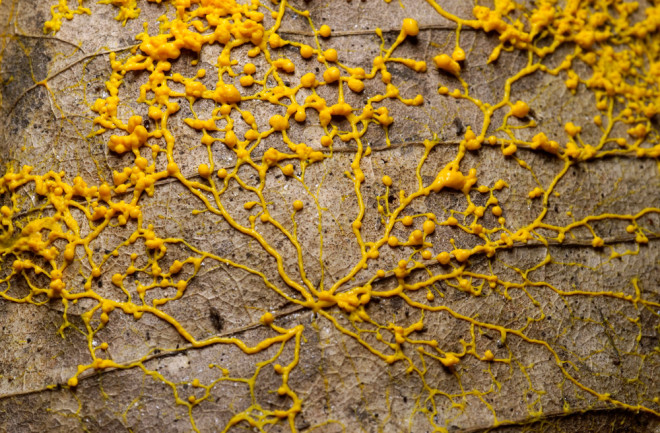
\includegraphics[width=0.4\textwidth]{Slime_Mould}
    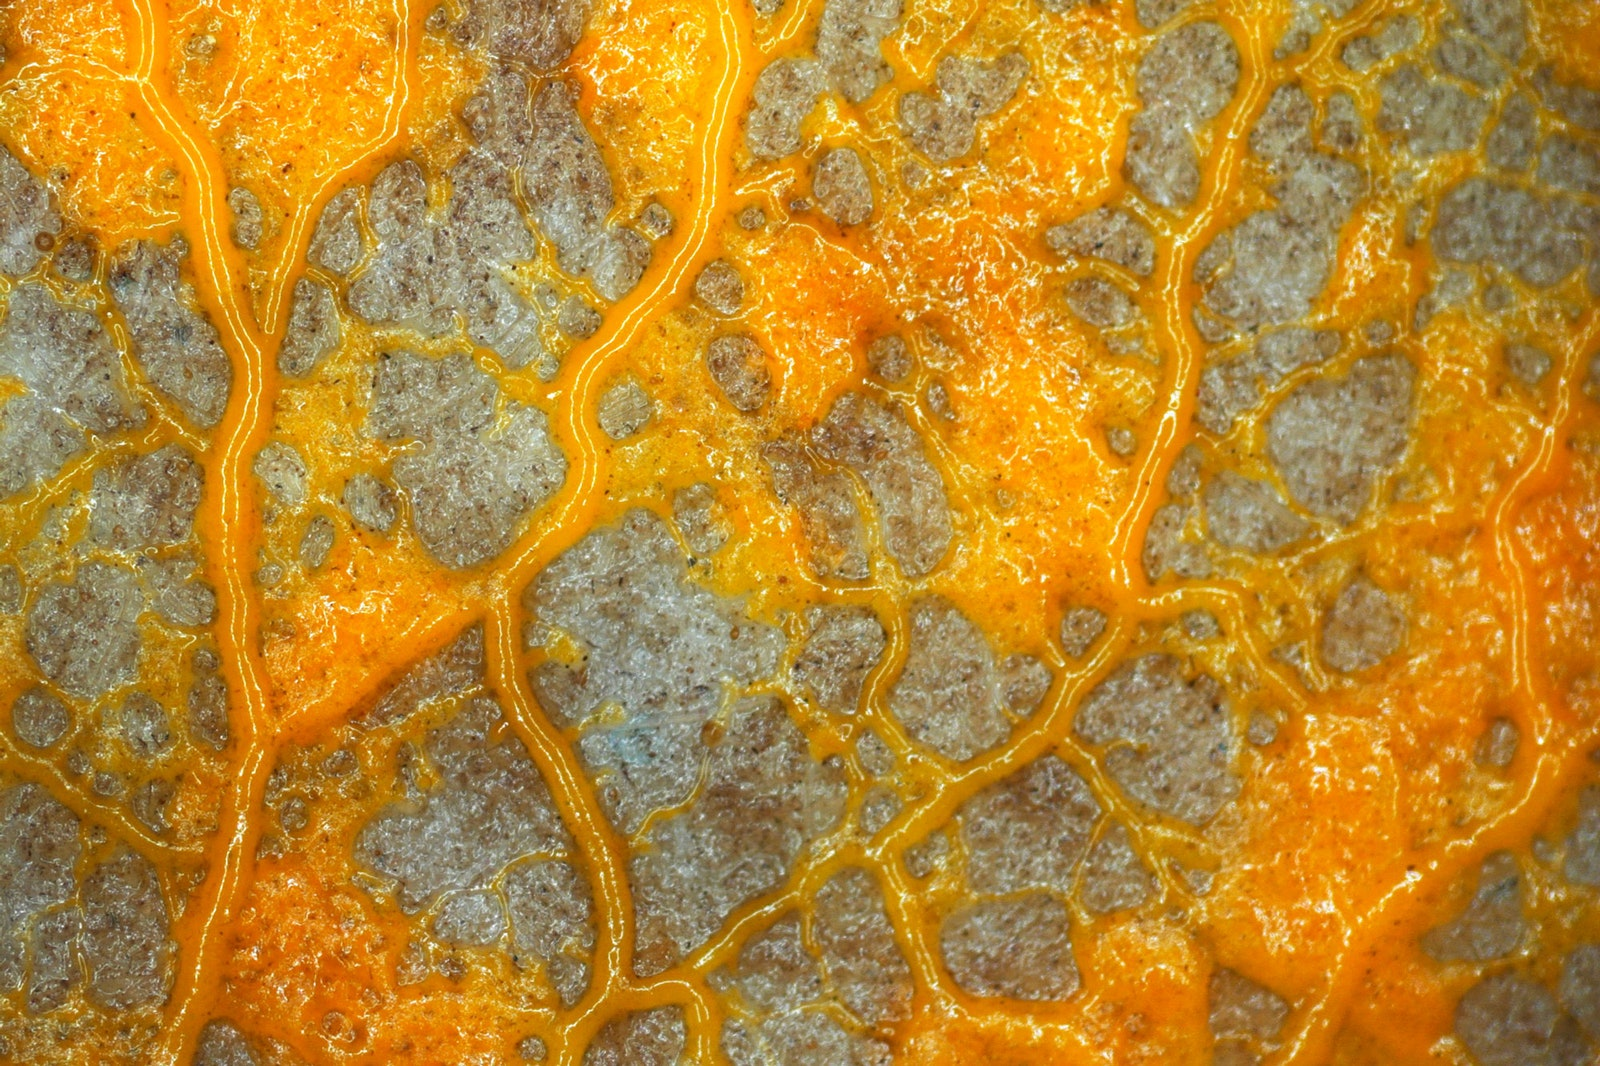
\includegraphics[width=0.4\textwidth]{Slime_Mould2}
    \caption{Many species of slime moulds are known for their ability to `solve' complex problems, such as mazes or even travelling salesman puzzles. This is especially remarkable as they really are individual organisms that work together in intricate ways through relatively simple chemical signalling.}
    \label{fig:my_label}
\end{figure}

\begin{enumerate}[label=(\alph*)]
    \item Explain why no-flux conditions for the cell density $n$ and chemoattractant concentration $c$ imply Neumann conditions on these quantities. 
    \sol{
    This is just noticing that the boundary condition on $c$ is Neumann, which means the extra term in the boundary condition on $n$ vanishes and hence $n$ satisfies a Neumann condition. So we have,
    $$
    \pd{n}{x} = \pd{c}{x} = 0, \quad x = 0,L.
    $$
    }
    \item Deduce that any positive real number $n^*>0$ is a feasible steady state for the cell density, and determine the corresponding value of the chemoattractant at such a steady state, $c^*$. What biological assumption did we make which allows this to happen (as opposed to having a fixed number of steady states)?
    \sol{
    This follows immediately as the only constraint for an equilibrium is that $an^* - bc^*=0$ and hence $c^* = an^*/b$ for any value of $n^*$. We need this to be positive for the state to be feasible. The assumption which led to this is that we can neglect growth or death of the cells, $n$. If we add a logistic term for example to the equation for $n$, then we pick out the two steady states given in the notes.
    }
    \item Using the equation for the cell density and the boundary conditions, show that the total mass of cells cannot change over time. 
    \sol
    {
    The total mass of cells is given by
    $$ M_n(t) = \int_0^L n(t,y)dy.$$
    Taking the derivative with respect to $t$ we find,
    $$
    \fd{M}{t} = \int_0^L \pd{n}{t}dy = \int_0^L D_n\pdd{n}{x} - \pd{}{x}  \left(n\chi \pd{c}{x}\right)dy =  \left [-D_n\pd{n}{x} + n\chi  \pd{c}{x}\right ]_{x=0}^{x=L} = 0,
    $$
    where we have used the Fundamental Theorem of Calculus and then noticed that we arrive at exactly the expression for the boundary conditions. Hence we have that $M(t)$ must in fact be a constant.
    }
    \item Linearize the system around the homogeneous equilibrium found above, treating the homogeneous cell density $n^*$ as a constant.
    \sol{
    The linearization is exactly as in Section 5.1.1 in the lecture notes, except without the logistic term in the first equation. Hence we have that perturbations satisfy,
    \begin{align*}
    \pd{N}{t} &= D_n\nabla^2 N - n^*\chi  \nabla^2 C, \\
    \pd{C}{t} &= D_c\nabla^2C + aN -  bC.
    \end{align*}
    }
    \item Using the usual ansatz that the perturbations are proportional to $e^{\lambda_k t} w_k(x)$, determine the quadratic equation that the growth rates $\lambda_k$ satisfy in terms of the Laplacian eigenvalues $\rho_k$. You do not need to compute the $w_k$ or $\rho_k$ (though they should be straightforward to compute!)
    \sol{Using the suggested ansatz, again as in Section 5.1.1, we find the growth rates satisfy the linear algebraic system,
        \begin{align*}
    \lambda_kN  &= -D_n\rho_kN + n^*\chi  \rho_kC , \\
    \lambda_kC &= -D_c\rho_kC + aN -  bC.
    \end{align*}
    Equivalently, the $\lambda_k$ are eigenvalues of,
    $$
    \m{M} = \begin{pmatrix}
    -D_n \rho_k & n^*\chi  \rho_k\\ a & -b-D_c \rho_k
    \end{pmatrix}
    $$
    So we have that the growth rates satisfy,
    \begin{equation}\label{lambda_k}
    \lambda_k^2 +(\rho_k(D_n+D_c)+b)\lambda_k+(D_n(b+D_c\rho_k)-n^*\chi a)\rho_k=0.
    \end{equation}
    }
    \item Using the quadratic above, show that the inequality,
    $$
    n^* > \frac{D_n b}{\chi a},
    $$
    is necessary for a pattern-forming instability to occur. What key assumption do we need to deduce this inequality, and what does this assumption mean in terms of the domain length $L$?
    \sol{
    We see that the trace of $\m{M}$ is always negative, and hence the coefficient of $\lambda_k$ in \eqref{lambda_k} will always be positive. Hence the only possibility for growth rates with positive real part is if $h(\rho_k) = \det(\m{M}) = D_nD_c\rho_k^2+(D_nb-n^*\chi a)\rho_k<0$ for some $\rho_k$. As in Section 5.1.1, we can find the minimum by computing,
    $$
    \fd{h}{\rho_k} = 2D_nD_c\rho_k^*+(D_nb-n^*\chi a)=0 \implies \rho_k^* = \frac{n^*\chi a-D_nb}{2D_nD_c}.
    $$
    To ensure $\rho_k^*>0$, we must have $n^*\chi a-D_nb>0$. Substituting this in we find,
    $$
    h(\rho_k^*) = \frac{(D_nb-n^*\chi a)^2}{4D_nD_c} - \frac{(D_nb-n^*\chi a)^2}{2D_nD_c} = -\frac{(D_nb-n^*\chi a)^2}{4D_nD_c}<0,
    $$
    and hence the minimum is always negative. So the only requirement from the above for $h(\rho_k)$ to be negative is that $n^*\chi a-D_nb>0$ or, equivalently, 
    $$n^* > \frac{D_n b}{\chi a}. $$
    
    \textbf{Alternatively:} One could also spot that $h(x)$ is a quadratic in $x$ of the form $Ax^2+Bx$, and so for this to have negative values for positive $x$ we must have $B/A<0$. 
    
    The key assumption in the above is that we can approximate the Laplace eigenvalues $\rho_k$ as continuous, which is valid for $L \gg 1$.
    }
    \item (Optional) In the absence of the transport terms (equivalently, for $\rho_0=0$), does it make sense to consider the steady state you found in part (b) stable? Hint: Does it make sense to consider perturbations with $\rho_0=0$, given the results you've found in part (c)?
    \sol{
    If we allowed perturbations with $\rho_0=0$, these would be constant in space. By our equation for $\lambda_k$ above these would satisfy,
    $$
    \lambda_0^2 +b\lambda_0=0 \implies \lambda_0=-b, 0.
    $$
    Hence, strictly speaking, these would be in the degenerate case where we cannot deduce their stability due to a zero growth rate. However, such constant perturbations would violate the conservation of mass shown in (c), as they would change $M$. So if we think only of perturbations respecting a given mass $M$, then we do not consider $k=0$ a permissible mode.
    }
\end{enumerate}




\iffalse
\begin{equation}
\label{sys1}
\begin{aligned}
\pd{u}{t}  &= \pdd{u}{x} + u(1-u)-g\left(\frac{u}{v}\right)v,\\
\pd{v}{t}  &= D\pdd{v}{x} + g\left(\frac{u}{v}\right)v-av.
\end{aligned}
\end{equation}
\fi
    
    
\end{document}